\begin{wrapfigure}{l}{0.1\textwidth}
	\vspace{-10pt}
	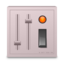
\includegraphics[width=\linewidth]{images/ikony_unitytweaktool.png}
\end{wrapfigure}

W \textcolor{ubuntu_orange}{Ustawieniach systemu} możesz do pewnego stopnia skonfigurować wygląd i zachowanie Unity, jednakże łatwo dostępne opcje są bardzo ograniczone. Zwiększenie możliwości konfiguracji wymaga zainstalowania dodatkowych narzędzi. Wspomniany wcześniej Menadżer Ustawień CompizConfig jest bardzo potężnym narzędziem konfiguracyjnym, ale mnogość opcji może przerażać. CCMS pozwala zmodyfikować nie tylko Unity, ale całość wyglądu systemu.

Prostszym narzędziem, dedykowanym środowisku Unity, jest \textcolor{ubuntu_orange}{Unity Tweak Tool}. Program możesz zainstalować za pomocą Centrum Oprogramowania Ubuntu lub przy pomocy konsoli:
\begin{lstlisting}[language=bash]
sudo apt-get install unity-tweak-tool
\end{lstlisting}
